\section{Általánosított diszkrét maximum-elv magasabbrendű elemekre}\label{sec:general_DMP}

Ebben a szakaszban az 1 dimenziós Poisson-egyenlet végelselemes approximációját vizsgáljuk.  Először egy ellenpéldán keresztül igazoljuk, hogy a klasszikus diszkrét maximum-elv nem terjeszthető ki a magasabbrendű végeselemes közelítésekre (hp-FEM). Ennek az az oka, hogy a jobb oldali $f$ függvény nempozitivitásából nem feltétlenül következik $l(.)$ korlátos lineáris funkcionál nempozitivitása. A probléma kiküszöbölésésre kimondjuk az általánosított diszkrét maximum-elvet, ami a nempozitivitást az $f$ függvény helyett annak $V_h$ térbeli $L^2$-vetületére feltételezi. Végül megmutatjuk, hogy az általánosított diszkrét maximum-elv  bizonyos feltevések mellett igazolható magasabbrendű közelítésekre is. A szakaszban bemutatott eredmények \cite{sol-vej}-ből származnak. 

Tekintsük az $\Omega = (a,b)\in \R$ intervallumon a $-u'' = f$ Poisson-egyenletet homogén Dirichlet-peremmel, azaz $u(a) = u(b) = 0$. Ez a korábban definiált \eqref{dirichlet_problem} feladatnak a $p \equiv 1 $ és $q \equiv 0$ esete. A gyenge feladat ekkor: adott $f \in L^2(\Omega)$ mellett keressük azt az $u \in H_0^1(\Omega)$ függvényt, amelyre
\begin{equation} \label{1dgyenge}
	\int_{a}^{b} u'(x)v'(x) \dd x =  \int_{a}^{b} f(x)v(x) \dd x, \quad (\forall v \in H_0^1(\Omega)).
\end{equation}

Tegyük fel, hogy $f \in L^2(\Omega)$, és osszuk fel  $\closure{\Omega}$-t $M$  darab szakaszra: $a = x_0 < x_1 < \ldots < x_M = b$. Ekkor a $\mathcal{T}_h$ trianguláció elemei a $T_k = [x_{k-1},x_k]$ intervallumok. A $V_h \subset H_0^1(\Omega)$ altér legyen most a
szakaszonként polinom függvények tere:
\begin{equation*}
	V_h = \left\{ u \in C(\closure{\Omega}): u|_{T_k} \in P^{p_k}, \forall T_k \in \mathcal{T}_h  \text{ és } u(a) = u(b) = 0 \right\}.
\end{equation*}

A végeselemes feladat tehát: keressük azt az $u_h \in V_h$ függvényt, amire teljesül a következő:
\begin{equation}\label{diszkret1d}
	\int_{a}^{b} u_h'(x)v_h'(x) \dd x =  \int_{a}^{b} f(x)v_h(x) \dd x, \quad (\forall v_h \in V_h).
\end{equation}

\begin{definition}
	\Aref({diszkret1d}) diszkrét feladatban jelölje az $f \in L^2(\Omega)$  függvény $V_h$ altérre vett $L^2$-vetületét $f_h \in V_h$ , ha $f_h$-ra teljesül:
	\begin{equation}\label{f_hdef}
		\int_a^b (f_h(x) - f(x)) v_h(x) \dd x = 0 \quad (\forall v_h \in V_h).
	\end{equation}
\end{definition}
\begin{remark}
	\Aref({f_hdef}) egyenletet átalakítva
	\begin{equation}
		\int_a^b f_h(x) v_h(x) \dd x  =  \int_a^b f(x) v_h(x) \dd x  = 0 \quad (\forall v_h \in V_h), 
	\end{equation}
	tehát a diszkrét feladat megoldásánál a tehervektort az $f$ és az $f_h$ függvényből számolva ugyanazt kapjuk.
\end{remark}

\subsection{Ellenpélda a klasszikus diszkrét maximum-elv kiterjesztésére magasabbrendű közelítésre}

Megmutatható, hogy \aref{cDMP}. klasszikus diszkrét maximum-elv már a harmadrendű végeselemek esetére sem terjeszthető ki, tehát amikor $u|_{T_k} \in P^{p}$, ahol $p = 3 \, (\forall T_k \in \mathcal{T}_h) $. Ennek bizonyításához tekintsük az Lobatto-polinomokat a $[-1, 1]$ intervallumon:
\begin{equation}\label{lobatto}
	l_k(x)= \int_{-1}^x L_{k-1}(\xi) \dd \xi, \quad 2 \leq k,
\end{equation}
ahol $L_{k-1}$ a normált $k-1$ fokú Legendre-poninomot jelöli. Ekkor $l_2, l_3, \ldots$ függvények $\pm 1$-ben $0$ értéket vesznek fel, és a $H_0^1$-beli skaláris szorzásra nézve ortonormáltak:
\begin{equation}\label{eq:legendre_on}
	\langle l_i, l_j \rangle_{H^1_0(\Omega)} = \int_{-1}^x l_i'(x)  l_j'(x) \dd x = \delta_{ij}, \quad 2 \leq i,j.
\end{equation}


\begin{example}\label{bukaspelda}
	Az $\Omega = (-1,1)$ intervallumon tekintsük a $\mathcal{T}_h = \{T_1\} = \{[-1,1]\}$ triangulációt. Harmadfokú közelítés esetén a $V_h$ altér bázisát alkotják az $l_2, l_3$ függvények, és a közelítő megoldás felírható $u_h = y_1 l_2(x) + y_2 l_3(x)$ alakban. Ekkor \eqref{eq:legendre_on} miatt a merevségi mátrix a $2 \times 2$ dimenziós egységmátrix, és az ismeretlen $y_1, y_2$ együtthatók felírhatók a következőképp:
	\begin{equation}
		y_i = \int_{-1}^1 \sum_{j=1}^2 y_i l_{j+1}'(x) l_{i+1}'(x) \dd x = \int_{-1}^1 f(x) l_{i+1}(x) \dd x, \quad i = 1,2.
	\end{equation}
	Legyen $f$ a következő: 
	\begin{equation}\label{eq:bukaspelda_rhs}
		f = 200 e^{-10(x+1)}.
	\end{equation}
	Ekkor az együtthatókra azt kapjuk, hogy:
	\begin{align*}
		y_1 & = -\sqrt{6}\frac{(9 + 11 e^{-20})}{10}, & y_2 & = \sqrt{10}\frac{(73 - 133 e^{-20})}{100}. 
	\end{align*}
	Tehát $u$-ra a végeselemes közelítés:
	\begin{equation}
		u_h(x) = \frac{1}{40} (1-x^2) (54 + 66 e^{-20} - (73 - 133 e^{-20})x). 
	\end{equation}
	\Aref{fig:solvejbukas} bal oldali ábrán látható, hogy $u_h$ negatív értékeket is felvesz az $\Omega$-n, tehát \aref{cDMP}. klasszikus diszkrét maximum-elv ekkor nem teljesül.
	
	 Ahhoz, hogy megértsük, miért nem igaz a feladatra \aref{cDMP}., vizsgáljuk meg az $f_h$ vetületet. Írjuk fel $f_h$-t az $l_2,l_3$ bázisfüggvények segítségével. Ezt \eqref{f_hdef}-be helyettesítve egy lineáris egyenletrendszert kapunk, amit megoldva:
	\begin{equation}
		f_h(x) = \frac{3}{80} (1-x^2) (110 e^{-20} + 90 + ( 931 e^{-20} - 511)x). 
	\end{equation}
	Ekkor, mint ahogy  \aref{fig:solvejbukas} jobb oldali ábrán megfigyelhető, $f_h$ negatív értékeket is felvesz az $\Omega$-n. Ez azt jelenti, hogy nem teljesül \aref({diszkret1d}) diszkrét feladatban a jobb oldal nemnegativitása vagyis nem teljesül a mátrix maximum-elv egyik feltétele.		
\end{example}

\begin{figure}[h]
	\centerline{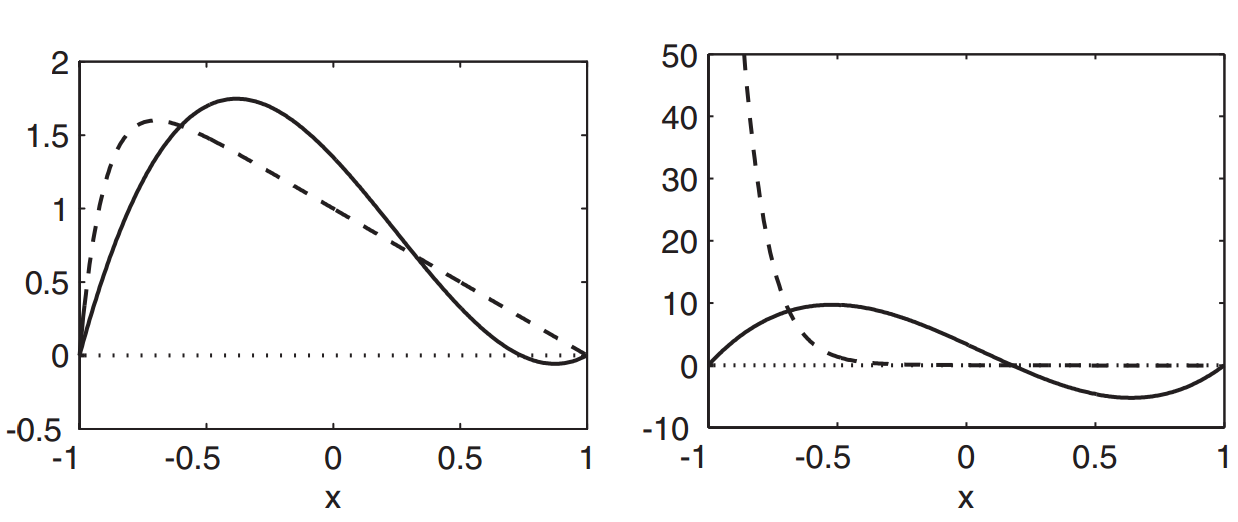
\includegraphics[width=.8\linewidth]{solvejbukas.png}}
	\caption{Bal oldalon: \aref{bukaspelda}. példa harmadfokú közelítése (folytonos vonallal), és a pontos megoldás (szaggatott vonallal). Jobb oldalon: az $f$ függvény \eqref{eq:bukaspelda_rhs} (szaggatottal), valamint az $f_h$ vetületi függvény (folytonos vonallal) \cite{sol-vej}. }
	\label{fig:solvejbukas}
\end{figure}

\subsection{Általánosított diszkrét maximum-elv}

\Aref{bukaspelda}. példabeli megfontolások alapján kimondható \aref{cDMP}. klasszikus diszkrét maximum-elv általánosabb megfelelője, ahol  $f$ helyett az $f_h$ vetületi függvényre adunk meg feltételt. A dolgozatban az általános diszkrét maximum-elvet csak a speciális alakú nempozitivitási illetve nemnegativitási elvként fogalmazzuk meg. Ebből következik az általánosabb eset is.


\begin{definition}\label{gDMP}
	Legyen az $f_h \in V_h$ az $f \in L^2(\Omega)$ függvény $L^2$-vetülete $V_h$-ra, amelyre \eqref{f_hdef} teljesül. Azt mondjuk, hogy \aref({diszkret1d}) diszkrét homogén Dirichlet-feladat kielégíti az általánosított diszkrét maximum-elvet, ha $\forall f_h \leq 0$ esetén $u_h \in V_h$ megoldásra:
	\begin{equation}\label{eq:gDMP}
		\max_{\closure{\Omega}} u_h \leq 0.
	\end{equation}	
\end{definition}

Az általánosított minimum-elv analóg módon megfogalmazható:

\begin{definition}\label{gDMinP}
	Legyen az $f_h \in V_h$ az $f \in L^2(\Omega)$ függvény $L^2$-vetülete $V_h$-ra, amelyre \eqref{f_hdef} teljesül. Azt mondjuk, hogy \aref({diszkret1d}) diszkrét homogén Dirichlet-feladat kielégíti az általánosított minimum-elvet, ha $\forall f_h \geq 0$ esetén $u_h \in V_h$ megoldásra:
	\begin{equation}\label{eq:gDMP}
		\min_{\closure{\Omega}} u_h \geq 0.
	\end{equation}	
\end{definition}


\begin{remark}
	\Aref{cDMP}. klasszikus diszkrét maximum-elvből következik \aref{gDMP}. általánosított diszkrét maximum-elv.
\end{remark}


A következőkben megmutatjuk, hogy \aref{gDMinP}. általánosított minimum-elv teljesül \aref({diszkret1d}) feladatra, ha van olyan kvadratúra formula, ami teljesít bizonyos feltételeket. 

\begin{definition}
	Legyenek $l_k(x), k\geq 2$ \aref({lobatto}) pontban definiált Lobatto-polinomok. Ekkor $(x,z) \in [-1,1]^2$ és $p\geq 1$ esetén definiálhatjuk a következő függvényeket:
	\begin{equation}\label{phipdef}
		\begin{aligned}
			\phi_1(x,z) &\coloneqq 0,& &\quad \text{ha } p = 1 \\
			\phi_p(x,z) &\coloneqq \sum_{k=1}^{p-1} l_{k+1}(x)l_{k+1}(z),& &\quad \text{különben}.
		\end{aligned}
	\end{equation}
\end{definition}

Ekkor $\phi_p$ a diszkrét Green-függvény \aref({diszkret1d}) feladatra a $\mathcal{T}_h = \{T_1\} = \{[-1,1]\}$ trianguláció mellett. Mivel $l_{i+1}(\pm 1) = 0$, minden $i \geq 1$ esetén, ezért 
	\begin{equation}
		\phi_p(x,z) = 0, \quad \forall (x,y) \in \partial \Omega,
	\end{equation}
	ahol $\partial \Omega$ továbbra is a peremet jelöli.
	
\begin{definition}
	Legyenek $\mathcal{K}_p^+ \subset [-1,1]^2$ és $\mathcal{K}_p^+(x) \subset [-1,1]$ minden $q \geq$ esetén a következő halmazok:
	\begin{align*}
		\mathcal{K}_p^+ &\coloneqq  \{ (x,z) \in [-1,1]^2 : \phi_p(x,z) \geq 0 \}, \\
		\mathcal{K}_p^+(x) &\coloneqq  \{ z \in [-1,1] : (x,z) \in  \mathcal{K}_p^+ \}.	
	\end{align*}	
\end{definition}

\begin{lemma}\label{szimmlemma}
	Minden $(x,z) \in [-1,1]^2$ és $p\geq 1$ esetén $\phi_p(x,z) = \phi_p(-x,-z) = \phi_p(z,x)$ teljesül.
\end{lemma}

\begin{proof}
	A $\phi_p(x,z) = \phi_p(z,x)$ szimmetria $\phi_p(x,z)$ \eqref{phipdef}. definíciójából  közvetlen adódik. A Legendre-polinomokról tudjuk, hogy paritásuk megegyezik a fokszámuk paritásával, és ez \eqref{lobatto} miatt $l_k(x)$ függvényekre is teljesül. Ekkor	
	\begin{equation*}
		\phi_p(x,z) = \sum_{k=1}^{p-1} l_{k+1}(x)l_{k+1}(z) = \sum_{k=1}^{p-1} l_{k+1}(-x)l_{k+1}(-z) = \phi_p(-x,-z), \quad \forall p \geq 1.
	\end{equation*}	
\end{proof}

\begin{theorem}\label{fottetel}
	Legyen $\Omega = (a,b) \subset \R$. Tekintsük \aref({diszkret1d}) feladatot a $\mathcal{T}_h = \{ T_1, \ldots, T_M\}$ trianguláció, és $p_1, \ldots, p_M$ fokszámok mellett. Ha $\forall p \in \{p_1, \ldots, p_M \}$  valamint $\forall x \in (-1,1)$ esetén $\exists \mathcal{L}_{2p}(x)$ kvadratúra folrmula úgy, hogy:
	\begin{enumerate}[label=(\roman*)]
		\item 	$\mathcal{L}_{2p}(x)$ pontos a $2p$ fokú polinomokra $[-1,1]$-ben, \label{lpontos}
		\item	$\mathcal{L}_{2p}(x)$-hoz a súlyok nemnegatívak,
		\item	$\mathcal{L}_{2p}(x)$ minden alappontja $\mathcal{K}_p^+(x)$-beli. \label{lutolsó}
	\end{enumerate}
	Ekkor \aref({diszkret1d}) feladat kielégíti \aref{gDMinP}. általánosított minimum-elvet, és így \aref{gDMP}. általánosított maximum-elvet is.
\end{theorem}

\begin{proof}
	Tekintsük \aref({1dgyenge}) feladat $u \in H_0^1(\Omega)$ megoldását adott $f \in L^2(\Omega)$ mellett. Legyen az $f_h \in V_h$ az $f \in L^2(\Omega)$ függvény $L^2$-vetülete $V_h$-ra, amelyre \eqref{f_hdef} teljesül. Ekkor az $u_h \in V_h$ közelítés a következő formulával adott:
	\begin{equation*}
		\int_{a}^{b} u_h'(x)v_h'(x) \dd x =  \int_{a}^{b} f(x)v_h(x) \dd x = \int_a^b f_h(x) v_h(x) \dd x , \quad (\forall v_h \in V_h).
	\end{equation*}
	Vezessük be a következő kiegészítő folytonos problémát: keressük az $\tilde{u} \in H^1_0(\Omega)$ függvényt, amelyre
	\begin{equation*}
		\int_{a}^{b} \tilde{u}'(x)v'(x) \dd x =  \int_a^b f_h(x) v(x) \dd x , \quad (\forall v \in H^1_0(\Omega)).
	\end{equation*}
	
	Az egydimenziós Laplace-egyenlet megoldásának lineáris végeselsmes közelítése pontos minden osztópontban, és ez a tulajdonság magasabbrendű közelítésekre is igazolható (lásd: \cite{sol-seg}). Emiatt teljesül	
	\begin{equation*}
		u_h(x_i) = u(x_i) = \tilde{u}(x_i), \quad  i = 0, 1, \ldots, M.
	\end{equation*}
	A folytonos minimum-elv miatt $\tilde{u}(x_i) \geq 0$ az $\Omega$-n, így $u_h(x_i) \geq 0$, minden $i = 0, 1, \ldots, M$ esetén, ezért a tételt elég a $T_1 = \closure{\Omega}$ esetre belátni, ahol $\Omega = (-1,1)$.
	
	Az $u_h \in V_h$ megoldást a következő alakban keressük:
	\begin{equation}\label{1duh_linkomb}
		u_h = \sum_{i = 1}^{p-1} y_i l_{i+1}(x).
	\end{equation}
	
	\begin{equation*}
		y_i = \int_{-1}^1 f_h(z)l_{i+1}(z) \dd z, \quad  i = 1, 2, \ldots, p-1.
	\end{equation*}
	Ezt behelyettesítve \eqref{1duh_linkomb} egyenletbe
	\begin{equation}\label{uronda}
		u_h = \sum_{i = 1}^{p-1} \left( \int_{-1}^1 f_h(z)l_{i+1}(z) \dd z \right) l_{i+1}(x) = \int_{-1}^1 f_h(z) \phi_p(x,z) \dd z, 
	\end{equation}
	ahol $\phi_p(x,z)$ \aref({phipdef}) szerinti.
	
	Rögzítsük az $x \in (-1,1)$ pontot, és tegyük fel, hogy $\exists \mathcal{L}_{2p}(x)$ kvadratúra formula $z_0, \ldots, z_{2p} \in \mathcal{K}_p^+(x)$ pontokkal és $w_0, \ldots, w_{2p}$ nemnegatív súlyokkal. Az  $f_h(z) \phi_p(x,z)$ szorzatról tudjuk, hogy legfeljebb $2p$-edfokú polinom $z$-ben tetszőleges rögzített $x$ esetén, ezért \ref{lpontos}-ból $\mathcal{L}_{2p}(x)$ pontos minden $f_h(z) \phi_p(x,z) $-re. Ekkor \eqref{uronda} miatt 
	\begin{equation}\label{alsobecsles}
		u_h = \int_{-1}^1 f_h(z) \phi_p(x,z) \dd z = \sum_{i = 0}^{2p} \underbrace{w_i}_{\geq 0} \underbrace{f_h(z_i)}_{\geq 0} \underbrace{\phi_p(x,z_i)}_{\geq 0} \geq 0,
	\end{equation}
	ahol $w_i$ és $f_h(z_i)$ nemnegativitása a  feltevésekből adódik, $\phi_p(x,z_i) \geq 0$ pedig $z_i \in \mathcal{K}_p^+(x)$ miatt teljesül. Tehát \eqref{alsobecsles} pontból következik, hogy $u_h(x) \geq 0$ minden $x \in (-1,1)$ esetén, és így $u_h$ a $\partial \Omega$ peremen felveszi minimumát, tehát \ref{gDMinP}. teljesül. 
	
\end{proof}

A $p=2,4,6$ esetekben belátható, hogy $\phi_p(x,z) \geq 0$ minden $(x,z) \in [-1,1]^2$,  így ezekben az esetekben \aref{cDMP}. klasszikus diszkrét maximum-elv is igazolható. \Aref{gDMP}. általánosított diszkrét maximum-elv teljesülésének igazolásához minden más $p \geq 2$ esetre mutatnunk kell olyan kvadratúra formulát, amelyre \aref{fottetel}. tételbeli \ref{lpontos}-\ref{lutolsó} feltételek teljesülnek. \Aref{szimmlemma}. lemmabeli szimmetria miatt elegendő, ha az $x\in [0,1)$-en találunk ilyen kvadratúra formulákat. \Acite{sol-vej} 6. részében mutatnak példát a feltételeket kielégítő kvadratúra formulák konstuálására $p \leq 10$ esetekre.

